%
% Copyright (c) 2011-2013, fortiss GmbH.
% Licensed under the Apache License, Version 2.0.
% 
% Use, modification and distribution are subject to the terms specified
% in the accompanying license file LICENSE.txt located at the root directory
% of this software distribution. A copy is available at
% http://chromosome.fortiss.org/.
%
% This file is part of CHROMOSOME.
%
% $Id$
%

% =================================================================
\section{Example 3: Plug~\&~Play Showcase (30 minutes)}
\label{sec:example_pnp}
% =================================================================

In Section~\ref{sec:architecture}, we shortly explained the planned plug~\&~play features of \xme.
The current version implements both plug~\&~play and login features.
The following showcase illustrates the current state of plug~\&~play implementation.

This example is again based on the previous sensor/monitor example and extends it.
The goal is to activate a new sensor component on a third node called ''\emph{emptyNode}'' and a new monitor on a fourth node called ''\emph{monitorKB}''.
The \emph{emptyNode} is targeted to demonstrate the plug~\&~play and login capabilities in \xme, while \emph{monitorKB} is targeted to demonstrate 
the attribute support during plug~\&~play phase. 

In this case, we will use attributes to demonstrate data filtering during plug~\&~play phase of \xme. For this purpose, we differentiate
between the \emph{monitorNode}, containing one \emph{monitorB} component that filters sensing data received with the measurement unit
established to \emph{bytes}, and one \emph{monitorKB} component that filtering data measured in \emph{kilobytes}.

Hence, after the plug~\&~play phase is finished, the \emph{monitorB} component on \emph{monitorNode} will receive values from the \emph{sensorB} component placed on
\emph{sensorNode}, and the \emph{monitorKB} component on \emph{monitorNode} is going to receive sensing data from \emph{sensorKB} component located on \emph{emptyNode}.
The first sensing data is measured in \emph{bytes}, while the latter is measured in \emph{kilobytes}.

Additionally, in order to demonstrate logout capabilities, it is explained how the system reacts to a node logout received from ''\emph{emptyNode}''. 


\subsection{Adding the emptyNode}

The \emph{emptyNode} is already defined in the deployment model.
Open the model with the \emph{XMT} tool to have a look at it\footnote{See previous example how to do this.}~--~compare Figure~\ref{fig:pnp_deployment}.
The assignment of nodes to components is as follows:
\begin{itemize}
	\item[] \textbf{monitorNode:} \emph{loginManager}, \emph{pnpManager}, \emph{pnpClient}, \emph{monitorB} (displays bytes) and \emph{monitorKB} (displays kilobytes).
	\item[] \textbf{sensorNode:} \emph{pnpClient} and \emph{sensorB}.
	\item[] \textbf{emptyNode:} \emph{pnpClient} and \emph{pnpTrigger}.
\end{itemize}

\begin{figure}[htpb]
	\centering
	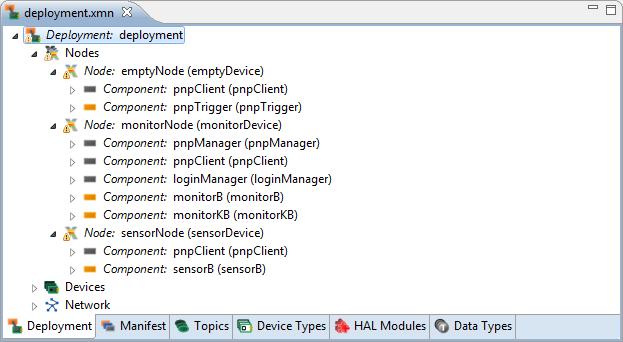
\includegraphics[width=0.9\textwidth]{figures/pnp_deployment.png}
	\caption{Deployment model highlighting the emptyNode.}
	\label{fig:pnp_deployment}
\end{figure}

The \emph{pnpTrigger} on \emph{emptyNode} is an example of a tutorial-specific component performing the following actions:
\begin{itemize}
	\item[] Requests the automatic instantiation of a \emph{sensorKB} component after the \emph{emptyNode} is logged-in.
	\item[] Request the logout of the \emph{emptyNode} after having demonstrated the other features. 
\end{itemize}

In this subsection, the objective is to demonstrate dynamic plug-in of the \emph{sensorKB} component. 
The latter will be demonstrated in the following subsection. 

%A \emph{Plug~\&~Play Client} component listens for commands to install and run new components on their node.\footnote{Currently this is only possible for the sensor and monitor components.}
%TODO: Remove from here and place it in the corresponding section (e.g. Architectures). 
%In future versions of \xme, the client will also be able to uninstall and transfer components from one node to another.

%The component which issues these commands is the \emph{Plug~\&~Play Manager}.

The \emph{Plug~\&~Play Manager} component exists at most once in a \xme network.
This component communicate with \emph{Login Manager} to provide authorization to establish connection between nodes that are already logged in.

%TODO: DISABLED FOR 0.6 REL, BECAUSE THE SCENARIO HAS CHANGED!
%The first step is sending a broadcast \emph{login request} message from the \emph{emptyNode}. The node owning the \emph{Login Manager}
%(currently \emph{monitorNode}) receives the request and process this request\footnote{In the future this will include credential, handshake or other
%security mechanisms to ensure that the requesting node can join to the network.}. 
%After checking credentials\footnote{Credential checking needs the modification of corresponding topic, and the existence of a credential checked in the system. This will be implemented in the future.}, 
%the \emph{Login Manager} communicates with the \emph{Plug~\&~Play Manager} to grant the access to the \emph{emptyNode}
%to create new components instances and the corresponding data links. 
%Finally, the \emph{Login Manager} sends a \emph{login response} to the \emph{emptyNode}. After receiving this login confirmation, 
%the \emph{emptyNode} will be able to publish its \emph{component instance manifest} with all components that it wants to deploy at runtime. 
%
%The \emph{Component Instance Manifest} is the topic exchanged between \emph{Plug \& Play Client} and \emph{Plug \& Play Manager}
%with the components already running on \emph{emptyNode} and the components that want to be deployed dinamically by the \emph{emptyNode}.
%In our case, we want to deploy dinamically one single components: a \emph{sensorKB} component. 
%Therefore this \emph{Component Instance Manifest} is sent from the \emph{Plug \& Play Client} running in the \emph{emptyNode} to
%the \emph{Plug \& Play Manager} running in the \emph{monitorNode}.
%
%When the \emph{Plug \& Play Manager} receives this \emph{Component Instance Manifest}, the Plug~\&~Play Manager checks this manifest and triggers the following components:
%\begin{itemize}
	%\item The \emph{Logical Route Manager} is asked for logically feasible routes between existing and new components.
	%\item The \emph{Network Configuration Calculator} is triggered for the logically feasible routes
		%in order to calculate transport mechanisms (\emph{waypoints}) for the logical routes (for example using UDP communication).
%\end{itemize}
%
%The respective outcome is then forwarded to the individual \emph{Plug~\&~Play Client} components in the affected nodes
%in order to implement the required changes.

%In this (preliminary) example, the command to activate the new sensor component is sent in the \texttt{\_step()} function of the Plug~\&~Play Manager.
%This code is already present, but has been commented out.
%We will reactivate it as follows:
%Open the following file:
%
%\begin{itemize}
%	\item[] \texttt{<XME\_ROOT>/examples/sensorMonitor/src/sensorMonitor/adv/pnpManager/src/}\\
%\texttt{pnpManagerFunction.c}.
%\end{itemize}
%At the top of the file, you will find the following code snippet:
%
%\begin{lstlisting}[breaklines]
%// PROTECTED REGION ID(SENSORMONITOR_ADV_PNPMANAGER_PNPMANAGERFUNCTION_C_INCLUDES) ENABLED START
%#include "xme/core/manifestRepository/include/manifestRepository.h"
%#include "xme/core/directory/include/plugAndPlayManager.h"
%\end{lstlisting}
%\vspace{-\baselineskip}
%\begin{lstlisting}[breaklines, backgroundcolor=\color{yellow}, escapechar=\%]
%//#define ENABLEPNP
%\end{lstlisting}
%\vspace{-\baselineskip}
%\begin{lstlisting}[breaklines]
%// PROTECTED REGION END
%\end{lstlisting}
%
%\noindent Change the line highlighted in yellow to (i.e., remove the slashes at the beginning of the line):

%\begin{lstlisting}[breaklines, backgroundcolor=\color{yellow}, escapechar=\%]
%#define ENABLEPNP
%\end{lstlisting}

%This is all you need to do to enable the plug~\&~play showcase.
%Now follow these steps to run it:
Refer to Section~\ref{sec:example_sensorMonitor} for instructions on how to set up the build environment and build the code.
To run this example, follow these steps:

\begin{enumerate}
	\item First start the \emph{monitorNode}. This node contains four key components relevant to plug~\&~play and login process:
		\begin{itemize}
			\item A \emph{monitorB} component, subscribed to any \emph{sensorData} topic sensing data measured in \emph{bytes}.
			\item A \emph{monitorKB} component, subscribed to any \emph{sensorData} topic sensing data measured in \emph{kilobytes}.
			\item A \emph{pnpClient} component, listening to requests from \emph{pnpManager} component.
			\item A \emph{pnpManager} component, which orchestrates the plugin process of additional components to the network, and communication with the \emph{loginManager}
			  to grant access to already logged in nodes.
			\item A \emph{loginManager} component, which receives requests broadcasted by \emph{Login Client} component and delivers login responses to nodes which requested to login.
		\end{itemize}
	\item Start the \emph{sensorNode}. The \emph{sensorNode} contains two components at startup:
		\begin{itemize}
			\item A \emph{pnpClient} component, listening to requests from \emph{pnpManager} in the network.
			\item A \emph{sensorB} component, emitting sensor data in \emph{bytes}.
		\end{itemize}
		Like in the previous examples, the \emph{sensorB} component will ask you which partition to monitor
		(compare Figure~\ref{fig:example_pnp_sensorNode}).
		Choose any partition that you want. This will initiate the data production on the sensor side.
		As we do not have yet any subscriber for the data, the data is not received by any other component.
	\item Finally, start the \emph{emptyNode}. This \emph{emptyNode} contains two components:
		\begin{itemize}
			\item A \emph{pnpClient} component, in charge of sending \emph{component instance manifests} and listening to requests from \emph{pnpManager}.
			\item A \emph{pnpTrigger} component, a tutorial-specific component to demonstrate over the time the plug-in of one sensor component and the logout of the \emph{sensorNode}.
		\end{itemize}
		%The \emph{emptyNode} is started with the \emph{pnpTrigger} that sends a plug~\&~play request after 5 execution cycles and 
		%a \emph{pnpClient} to send component instance manifests to and to listening to requests from \emph{pnpManager}.
		%Notice that nothing is happening yet (the console window stays blank), because there exists no \emph{pnpManager} component sending requests to this node.
\end{enumerate}	
		
The logical steps when \emph{emptyNode} is running are as follows:
\begin{enumerate}
	\item After five execution cycles, the \emph{pnpTrigger} calls a function in the \emph{pnpClient} to trigger the initiate the plug-in process for a \emph{sensorKB} component in the \emph{emptyNode}.
	\item The \emph{pnpClient} on \emph{emptyNode} sends a \emph{Component Instance Manifest} topic message to the \emph{pnpManager} on \emph{monitorNode}
		to request that the \emph{sensorKB} component should be added.
	\item The \emph{pnpManager} receives the \emph{Component Instance Manifest} and process its content.
	\item The \emph{pnpManager} component calculates internally matches between subscriptions and publications with the
		current registered nodes and components (compare Figure~\ref{fig:example_pnp_monitorNode}). Additionally, for every matching topic,
		the attribute filter in subscription should match with attribute definitions associated to that topic in publications.
	\item A logical and physical route is calculated by the \emph{pnpManager} component, and the result is sent to the corresponding nodes.
	  In our case, the logical route for the \emph{sensorData} topic between the \emph{sensorKB} component specification on \emph{emptyNode}
		and the \emph{monitorKB} running component on \emph{monitorNode} is returned back as the result of plug~\&~play process.
	\item After receiving the \emph{runtime graph} topic on \emph{emptyNode}, the \emph{sensorKB} component is scheduled and starts running and ask you which partition to observe.
		Choose any partition~--~preferably other different partition than the other selected on \emph{sensorNode}.
		After this, the data production for \emph{sensorData} topic is delivered.
	\item After receiving the \emph{runtime graph} topic on \emph{monitorNode}, the \emph{monitorKB} component is scheduled and starts running receiving \emph{sensorData} expressed in \emph{kilobytes}.
	\item After this, both sensors (i.e., \emph{sensor ~--~in bytes~--~ on \emph{SensorNode}} and the newly created \emph{sensor} ~--~in kilobytes~--~ on the (formerly) \emph{emptyNode})
		send their measurements to the \emph{monitorB} and \emph{monitorKB} components located on \emph{MonitorNode}.
		Check the \emph{monitorNode} console window.
\end{enumerate}

\begin{figure}[htpb]
	\centering
	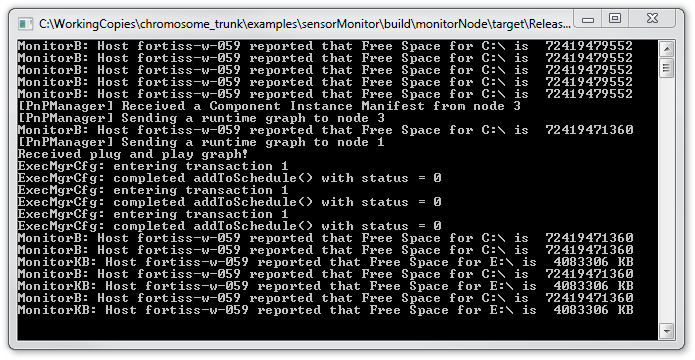
\includegraphics[scale=0.7]{figures/example_pnp_monitorNode.png}
	\caption{Console window of \emph{monitorNode} during plug~\&~play.}
	\label{fig:example_pnp_monitorNode}
\end{figure}

\begin{figure}[htpb]
	\centering
	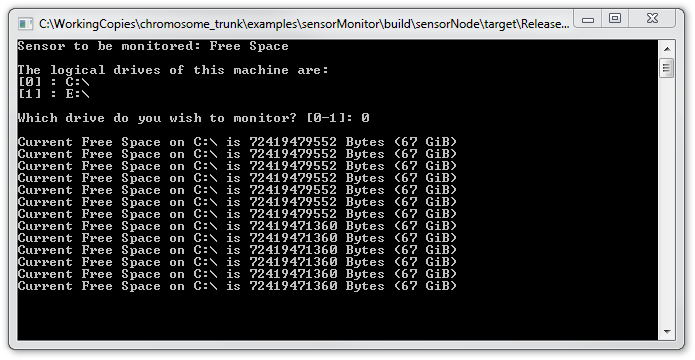
\includegraphics[scale=0.7]{figures/example_pnp_sensorNode.png}
	\caption{Console window of \emph{sensorNode}.}
	\label{fig:example_pnp_sensorNode}
\end{figure}

\begin{figure}[htpb]
	\centering
	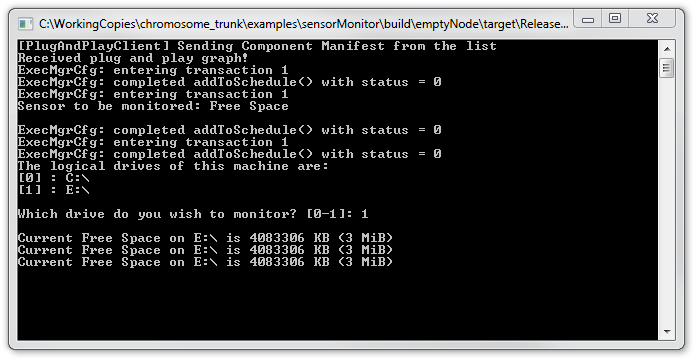
\includegraphics[scale=0.7]{figures/example_pnp_emptyNode.png}
	\caption{Console window of \emph{emptyNode} during plug~\&~play.}
	\label{fig:example_pnp_emptyNode}
\end{figure}

There is still one more node that can be added at runtime to the system, the \emph{lonelyNode}. 
We will explore how to integrate external nodes developed outside the common shared deployment model on \emph{XMT}.

\subsection{Self-initiated logout process for emptyNode}

In this subsection, it is explained the logout process for a given node, and how to communicate the logout of this node to other running nodes. 

This logout process for \emph{emptyNode} is a continuation of the execution of the plug-in example of the previous section. 
The responsible component for initiating the logout process is \emph{pnpTrigger}. The logout process will start after fifty execution cycles. 

For the execution of this example, it is expected that the user have already started the \emph{monitorNode}, the \emph{sensorNode} and the \emph{emptyNode}, as described in the previous section. 

The logout process for \emph{emptyNode} is executed as follows:
\begin{enumerate}
  % Step 0
	\item The \emph{pnpTrigger} requests to \emph{pnpClient} to trigger the logout process for the current node (in this case, the \emph{emptyNode}).
	% Step 1
	\item The \emph{pnpClient} generates a logout topic message. This logout topic message is delivered through the network to the \emph{pnpManager} on the \emph{monitorNode}.
	\item The \emph{pnpManager} receives the logout message with the node identifier. This will unannounce the node-associated componnent from \emph{pnpManager} (and thus, component ports from \emph{Logical Route Manager}, and calculates the logical routes to be removed. 
	\item At this point, there are two different set of logical routes:
	\begin{itemize}
		% Step 3.a
		\item The routes of subscribers obtaining data from the node to disconnect from \xme (\emph{emptyNode}). These nodes will receive a \emph{runtime graph} with the directive of removing all physical routes connected to the \emph{emptyNode}.
		% Step 3.b
	  \item The \emph{emptyNode} will receive all the connected physical routes (subscribers and publishers) to other nodes. 
	\end{itemize}
	\item The \emph{pnpClient} components in another nodes than \emph{emptyNode}, will reconfigure the scheduling to eliminate the subscription listening coming from \emph{emptyNode} and the publication of messages targeted to \emph{emptyNode}.
	\item The \emph{pnpClient} component in \emph{emptyNode}, will receive the confirmation that it can be disconnected safely from \xme. Before this complete disconnection, removes all schedules associated to publications and subscriptions, and sends an acknowledgement signal back to \emph{pnpManager}.
\end{enumerate}
		
\subsection{Third-party initiated logout process for sensorNode}

The logout process for \emph{sensorNode} is executed in the same was as the logout process in \emph{emptyNode}, with the difference which the process is directly triggered from \emph{pnpTrigger} component in \emph{monitorNode}. The logout process from \emph{pnpTrigger} will start after the seventieth execution cycle. This \emph{pnpTrigger} on \emph{monitorNode} calls directly the logout function in the \emph{pnpManager} to initiate the logout for node \emph{sensorNode}. The following steps are equal to the previous logout process. 

In this section, it was demonstrated how to connect and execute non-previously defined components in \xme (plug~\&~play), and how to disconnect nodes from the infrastructure at runtime (node logout). 